\documentclass[a4paper, 12pt]{article}
\usepackage{graphicx}
\usepackage{enumitem}
\usepackage{mathtools}
\usepackage{hyperref}
\usepackage{caption}
\usepackage{subcaption}
\def\code#1{\texttt{#1}}
\def\f#1{Figure \ref{fig:#1}}
\begin{document}

\title{\vspace{4.0cm}Reflections and Experiences with OpenCL\\
\large KTH DD2360 HT20}
\author{Pontus Asp}
\date{\today}
\maketitle
\thispagestyle{empty}
\pagenumbering{roman}
\newpage

\clearpage
\pagenumbering{arabic}

% Write here ->

% For this final exercise, kindly write a summary (max 1 A4 page) of your reflections and experiences with OpenCL, particularly when contrasting them against CUDA. Include atleast the following two discussion points:
%
%   * Reflect on the useability and easy-of-use of OpenCL contra Nvidia CUDA
%
%   * Contrast the performance of OpenCL contra Nvidia CUDA. Was the performance of your written the same, or did you find any anomalies? If you did find any anomalies, what could have caused these?
%
\section{Exercise 4}


% Write here <--

\end{document}



%\begin{figure}
%  \centering
%  \begin{subfigure}{.5\textwidth}
%    \centering
%    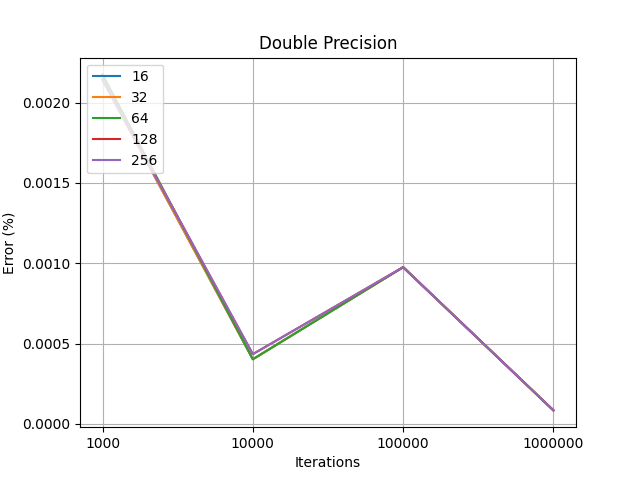
\includegraphics[width=1\linewidth]{graphs/ex_bonus_double_error.png}
%    \caption{Double Precision}
%    \label{fig:ex-single-double-error}
%  \end{subfigure}%
%  \begin{subfigure}{.5\textwidth}
%    \centering
%    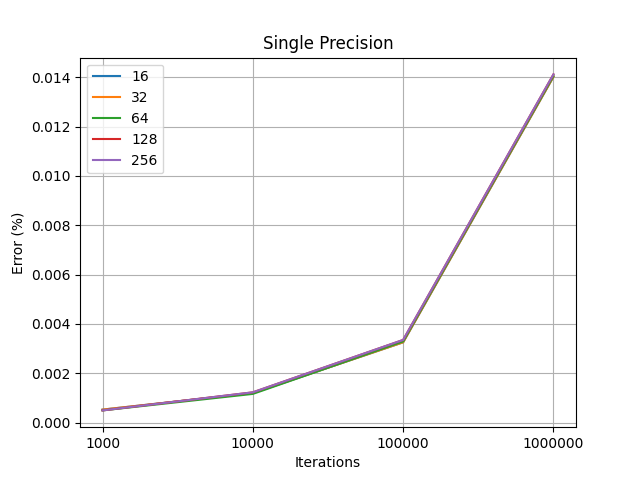
\includegraphics[width=1\linewidth]{graphs/ex_bonus_single_error.png}
%    \caption{Single Precision}
%    \label{fig:ex-bonus-single-error}
%  \end{subfigure}
%  \caption{Graphs of error using double and single precision with different amounts of iterations and block sizes.}
%  \label{fig:fig:ex-bonus-error}
%\end{figure}